\section{Proof Strategy}
We show that given a Coq model of both symbolic execution and the backwards symbolic execution tool and a set of properties, 
the backwards symbolic execution tool will give us a list of symbolic execution trees with corresponding leaves that, when executed, will result in an error state.

In other words, we define a list of symbolic execution trees, called \textit{tree\_list}, the we bind with a set of properties and a method to execute the relevant leaves, called \textit{execute\_tree\_list},
and show that it leads to a set of error states, called \textit{error\_states}. This can be expressed as the following theorem


\begin{theorem}[Correctness of Recursive Strategy]
\label{thm:sufficiency}
$execute\_tree\_list (tree\_list) \in error\_states$.
\end{theorem}
 
 In order to prove this, we first prove the following theorem:

\begin{theorem}[Execution ends in leaf of the last tree]
\label{thm:etl}
 $execute\_tree\_list (tree\_list) \in concretize\_leaf (t)$, where $t$ is the last element of $tree\_list$.
\end{theorem}

We then show that $concretize\_leaf (t) \in error\_states$, giving us our result.

We prove Theorem \ref{thm:etl} by induction. 
For our base case, we show that if the list only contains one tree, execution of that tree's root node with input specified by a selected leaf will result in an element of $concretize\_leaf (t)$.

\begin{figure}
\centering
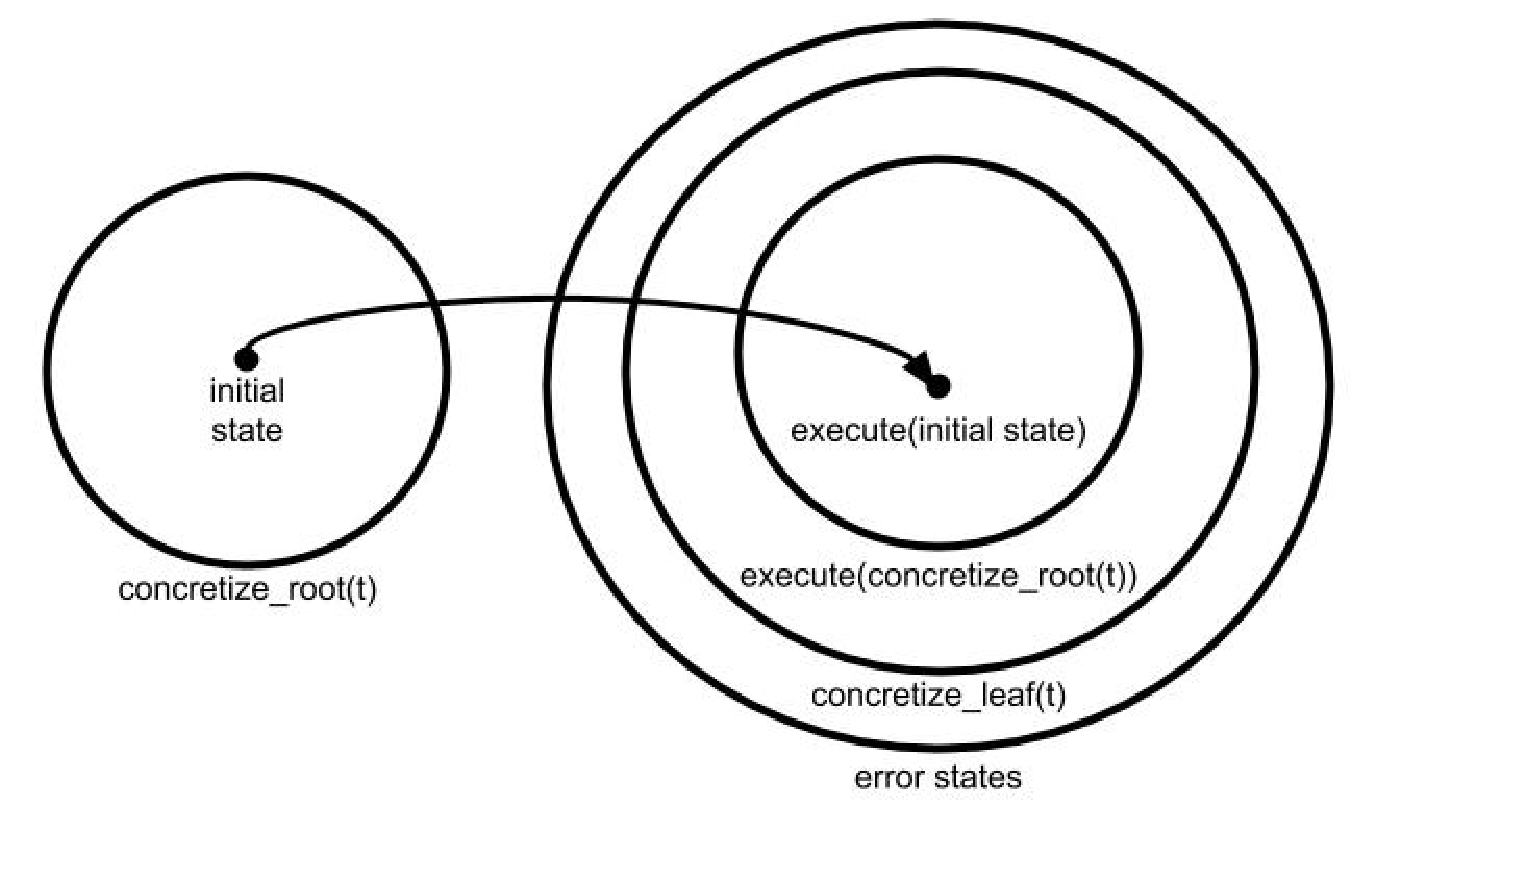
\includegraphics[width=.8\textwidth]{set3.eps}
\caption{Visual depiction of the base case of the proof.}
\label{fig:basecase}
\end{figure}

In other words, as depicted in Figure \ref{fig:basecase}, we show that the initial state is an element of $concretize\_root(t)$ of the tree, $t$, and that concretely executing any element of $concretize\_root(t)$ will result n an element inside $concretize\_leaf(t).$



For our inductive step, as depicted in Figures  \ref{fig:tlist} and \ref{fig:indstep}, we show that execution of each root with inputs from each specified leaf in a tree list of size $n$ will result in an element of $concretize\_leaf(t_n)$.

Our inductive hypothesis is that $execute\_tree\_list (tree\_list') \in concretize\_leaf (t_{n-1})$, where $tree\_list'$ is a $tree\_list$ with the last element removed. We then show that $concretize\_leaf (t_{n-1}) \subseteq concretize\_root (t_{n}) $, and therefore the concrete execution of any element in $concretize\_leaf (t_{n-1}) $ is in the set of of the concrete execution of any element in $concretize\_root (t_{n})$. Next, we show that $concretize\_root (t_{n}) \subseteq concretize\_leaf (t_{n})$, giving us our result.
 
\begin{figure}
\centering
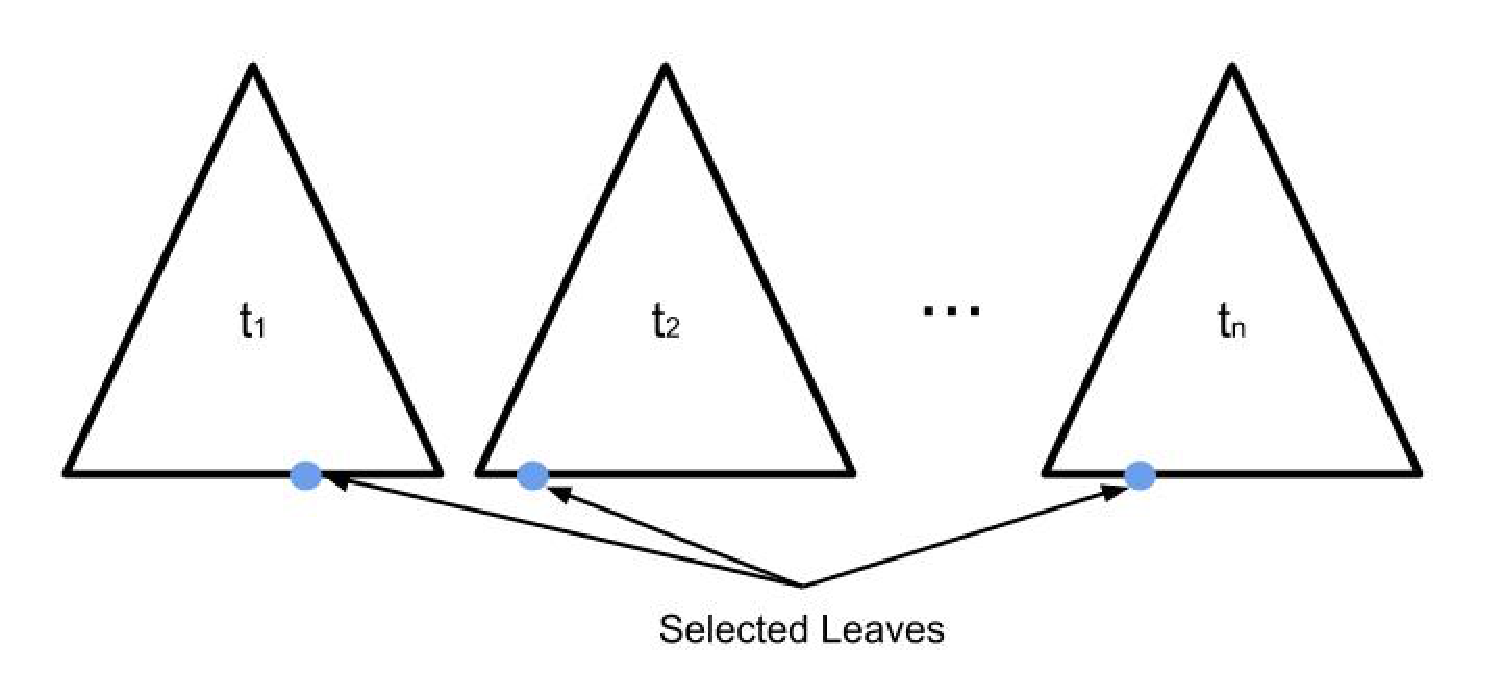
\includegraphics[width=.8\textwidth]{tlist.eps}
\caption{List of trees of length $n$.}
\label{fig:tlist}
\end{figure}

\begin{figure}
\centering
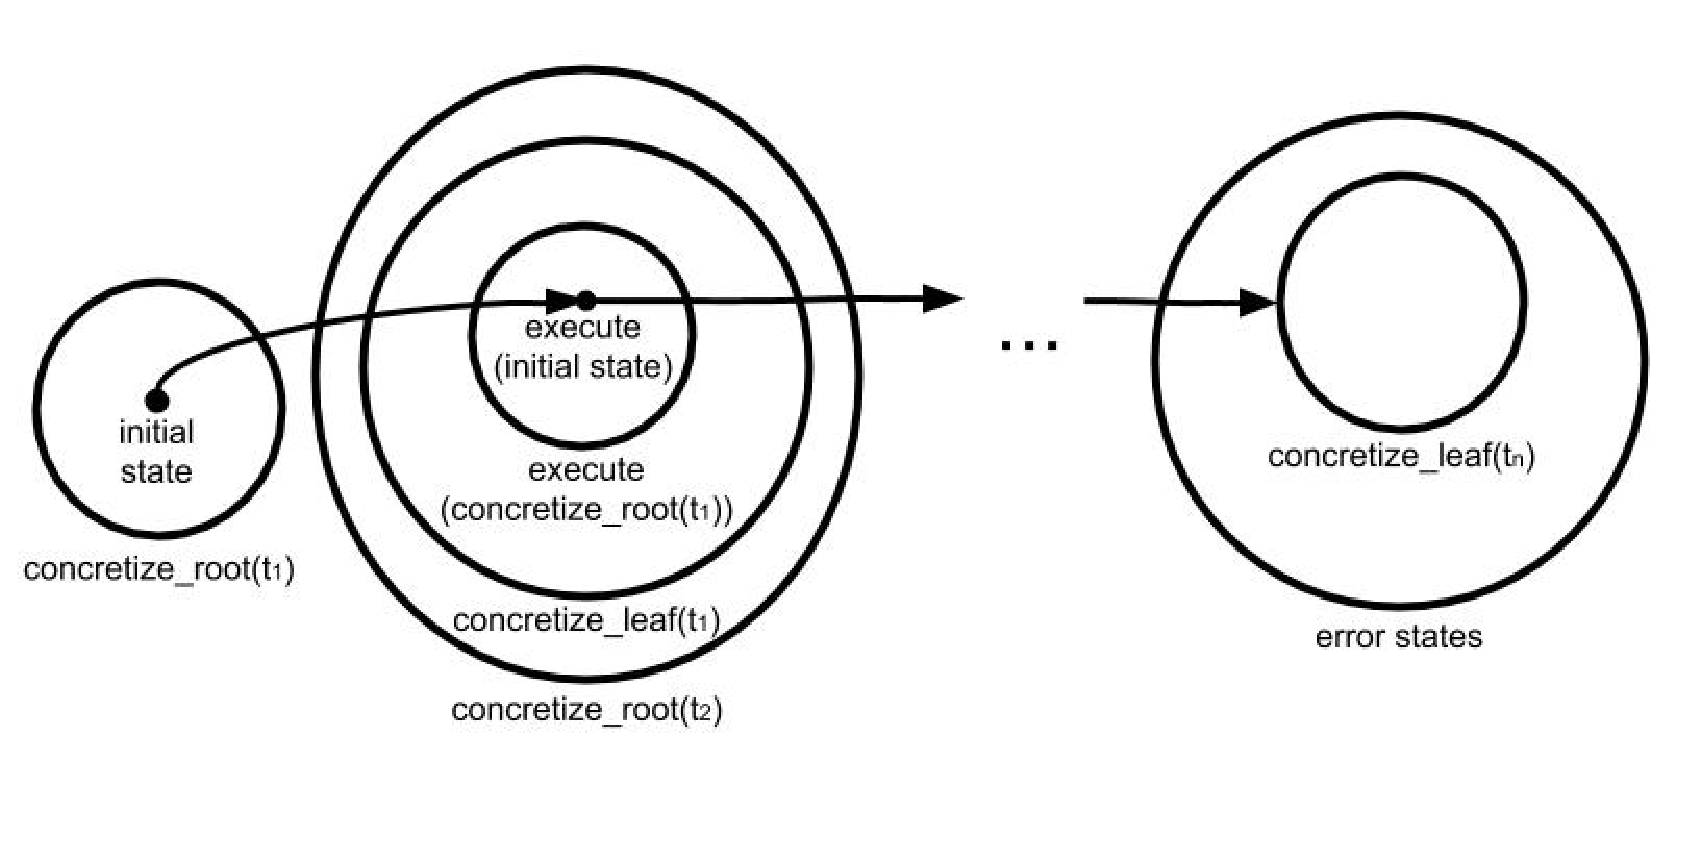
\includegraphics[width=.8\textwidth]{set4.eps}
\caption{Visual depiction of the inductive step of the proof.}
\label{fig:indstep}
\end{figure}
